% Section 12 of "Communication, Coherence and Collective Agents".
\section{Hierarchy: top-down priors and bottom-up evidence}\label{sec:hie}
% src: H2 (H2-D1, H2-D2, H2-P1 to H2-P14, H2-T1 to H2-T3, H2-L1, H2-L2, H2-X1, H2-X2, H2-E1 to H2-E3, H2-R1, H2-R2, H2-R4, H2-R5, H2-C1 to H2-C3, H2-O1 to H2-O6), H1-P2, H1-R10 to H1-R13, HC_critic V1 to V4, V13 and Sections 2 and 3, H6 (H6-P2, H6-P4, H6-C4, H6-P10), M_spec_H5 decisions 19 to 22 and Section 4

Hypothesis H5b concerns the passage between levels. A member can carry its collective as a latent cause whose prediction is an empirical prior on the member's own states, while the collective's state is estimated from what the members report. Reading a person's priors from a culture, an occupation or a community in this way is an interpretation, which \cref{rem:hie-gauge} develops. In hierarchical dynamic models the prediction of each level is an empirical prior on the level below, prediction errors ascend and predictions descend \citep{friston2008hierarchical}, and every factor of the joint model enters the free energy once. Among agents the top-down prior is often built from the receivers' own messages, a poll they answered or a record they wrote, and then a hierarchy can count the same evidence twice.

This section works in linear-Gaussian models, with discrete state spaces, nonlinear dynamics and renormalizing generative models left to remarks and open problems. It treats exact hierarchical messages (\cref{sec:hie-messages}), literal top-down reading (\cref{sec:hie-literal}), member-written records (\cref{sec:hie-records}), conformity to a self-constituted prior (\cref{sec:hie-conformity}) and three levels (\cref{sec:hie-three}); the member's model of its collective, the weight that records deserve and the open problems are in the Supplement (\cref{sec:hie-latent,sec:hie-balance,sec:hie-open}). Coarse variables follow \cref{def:met-coarse}, and every contrast is named: by default the precision-based contrast of \cref{def:col-contrast}, with record nodes where records are present, and for conventions, which have no world to condition on, contrast on their Gibbs precision.

The member's model of its collective as a latent cause is in the Supplement (\cref{sec:hie-latent}): without blanket input the members' process is a two-level model with an autonomous top level if and only if closure holds (\cref{prop:hie-closure-exact}), a Gaussian Markov model of the coarse coordinate alone is misspecified at a relative entropy rate no smaller than the stationary Markov defect (\cref{lem:hie-misspecification}), and under reversible drift contrast bounds the misspecification of an Ornstein--Uhlenbeck latent cause (\cref{prop:hie-reversible-sandwich}), each under the hypotheses stated there.

\subsection{Exact hierarchical messages on trees}\label{sec:hie-messages}

\begin{definition}[Gaussian tree model]\label{def:hie-tree}
A rooted tree with root $u_0$ carries Gaussian node variables $x_u$. The root has a proper prior with information $(\Lambda^\downarrow_{u_0},h^\downarrow_{u_0})$, $\Lambda^\downarrow_{u_0}\succ0$; every other node satisfies $x_u=\mathsf G_ux_{\mathrm{pa}(u)}+\mathfrak e_u$ with link noise $\mathfrak e_u\sim\Ncal(0,\Psi_u)$, $\Psi_u\succ0$, all independent; the data at $u$ enter through a likelihood $\exp(h^{\mathrm o\top}_ux_u-\frac12x_u^\top\Lambda^{\mathrm o}_ux_u)$, $\Lambda^{\mathrm o}_u\succeq0$, conditionally independent across nodes given the node variables. For sensing $o_u=H_ux_u+v_u$, $v_u\sim\Ncal(0,R_u)$, these are the information contributions $\Lambda^{\mathrm o}_u=H_u^\top R_u^{-1}H_u$ and $h^{\mathrm o}_u=H_u^\top R_u^{-1}o_u$ of \cref{prop:agy-consensus}. We write $\mathrm{pa}(u)$, $\mathrm{ch}(u)$ and $\mathcal T_u$ for the parent, the children and the subtree of $u$. A collective with members is the two-level tree whose root is $y_C$ and whose leaves are the members' states; a society of groups of members is a three-level tree.
\end{definition}
% src: H2-D2

\begin{theorem}[Exact messages: likelihoods up, leave-one-out priors down]\label{thm:hie-messages}
In \cref{def:hie-tree} define from the leaves up
\begin{equation}\label{eq:hie-up}
\begin{gathered}
\Lambda^{\mathcal T}_u=\Lambda^{\mathrm o}_u+\sum_{c\in\mathrm{ch}(u)}\Lambda^\uparrow_c,\qquad h^{\mathcal T}_u=h^{\mathrm o}_u+\sum_{c\in\mathrm{ch}(u)}h^\uparrow_c,\\
\Lambda^\uparrow_u=\mathsf G_u^\top(I+\Lambda^{\mathcal T}_u\Psi_u)^{-1}\Lambda^{\mathcal T}_u\mathsf G_u,\qquad h^\uparrow_u=\mathsf G_u^\top(I+\Lambda^{\mathcal T}_u\Psi_u)^{-1}h^{\mathcal T}_u,
\end{gathered}
\end{equation}
and from the root down $\Lambda^{\mathrm{post}}_u=\Lambda^\downarrow_u+\Lambda^{\mathcal T}_u$, $h^{\mathrm{post}}_u=h^\downarrow_u+h^{\mathcal T}_u$, the cavity $(\Lambda^{\mathrm{cav}}_{u\setminus c},h^{\mathrm{cav}}_{u\setminus c})=(\Lambda^{\mathrm{post}}_u-\Lambda^\uparrow_c,h^{\mathrm{post}}_u-h^\uparrow_c)$ with mean $m^{\mathrm{cav}}_{u\setminus c}$ for $c\in\mathrm{ch}(u)$, and $(\Lambda^\downarrow_c,h^\downarrow_c)$ the information of $\Ncal\bigl(\mathsf G_cm^{\mathrm{cav}}_{u\setminus c},\mathsf G_c(\Lambda^{\mathrm{cav}}_{u\setminus c})^{-1}\mathsf G_c^\top+\Psi_c\bigr)$. Then:
\begin{enumerate}
\item[(a)] $(\Lambda^{\mathcal T}_u,h^{\mathcal T}_u)$ is the information of the likelihood of the data in $\mathcal T_u$ given $x_u$, and $(\Lambda^\uparrow_u,h^\uparrow_u)$ that of the same data given $x_{\mathrm{pa}(u)}$: upward messages carry likelihoods, and no prior enters them;
\item[(b)] $(\Lambda^{\mathrm{post}}_u,h^{\mathrm{post}}_u)$ is the information of the exact posterior of $x_u$, the cavity that of $p(x_u\mid\text{data outside }\mathcal T_c)$, and $(\Lambda^\downarrow_c,h^\downarrow_c)$ that of $p(x_c\mid\text{data outside }\mathcal T_c)$: downward messages are leave-one-out priors;
\item[(c)] with $m^\downarrow_u$ the mean of the prior from above, $m^{\mathrm{post}}_u=m^\downarrow_u+(\Lambda^{\mathrm{post}}_u)^{-1}(h^{\mathcal T}_u-\Lambda^{\mathcal T}_um^\downarrow_u)$, where $h^{\mathrm o}_u-\Lambda^{\mathrm o}_um^\downarrow_u=H_u^\top R_u^{-1}(o_u-H_um^\downarrow_u)$ for direct data and $h^\uparrow_c-\Lambda^\uparrow_cm^\downarrow_u=\mathsf G_c^\top(I+\Lambda^{\mathcal T}_c\Psi_c)^{-1}(h^{\mathcal T}_c-\Lambda^{\mathcal T}_c\mathsf G_cm^\downarrow_u)$ for each child: every bottom-up contribution is a precision-weighted prediction error of the child's evidence relative to the parent's prior from above, and given that prior the prediction error and the likelihood message determine each other.
\end{enumerate}
\end{theorem}
% src: H2-T1; HC_critic V1

Proof in \cref{app:hie}; checked in \cref{chk:hie-messages}. Exactness of belief propagation on trees is due to \citet{pearl1988probabilistic}, cited for attribution, and the cavity is the provenance device of the channel filters of decentralized fusion \citep{grime1994data}. In the neuronal scheme of \citet{friston2008hierarchical} states are instead driven by precision-weighted prediction errors from their own level and the level below, and for continuous states belief propagation and variational message passing reduce to predictive coding \citep{friston2017graphical}.

On the Gaussian tree, predictive coding by gradient descent and coordinatewise mean-field message passing also converge to the exact posterior mean, under the conditions stated there (Supplement, \cref{prop:hie-predictive-coding}).

\subsection{Double counting by literal top-down reading}\label{sec:hie-literal}

A member whose prior is its collective's estimate, which already contains its own report, reads literally when it treats that estimate as independent of its own data: this is level-1 reading (\cref{def:fw-levels}) of a message whose provenance overlaps the receiver's data, with the collective's posted covariance as the law header, and its error is the overvaluation case of \cref{sec:mis}.

\begin{proposition}[One literal reading]\label{prop:hie-literal-once}
\begin{enumerate}
\item[(a)] In \cref{def:hie-tree}, a child $c$ of $u$ that takes as its prior the push-forward of the parent's full posterior through its link, and adds the likelihood of its subtree, claims the precision $\Lambda^{\mathcal T}_c+(\mathsf G_c(\Lambda^{\mathrm{post}}_u)^{-1}\mathsf G_c^\top+\Psi_c)^{-1}\succeq\Lambda^{\mathrm{post}}_c$, with equality only if $\mathsf G_c[(\Lambda^{\mathrm{cav}}_{u\setminus c})^{-1}-(\Lambda^{\mathrm{post}}_u)^{-1}]\mathsf G_c^\top=0$.
\item[(b)] In a scalar tree let a child $u$ of a parent $C$ have $\mathsf G_u=1$, $\Psi_u=\psi\ge0$ and subtree information $\mathsf J=\Lambda^{\mathcal T}_u>0$, let $\mathsf a=\Lambda^{\mathrm{post}}_C-\Lambda^\uparrow_u>0$ be the cavity precision, and put $\mathsf w=\Lambda^\uparrow_u/(\mathsf a+\Lambda^\uparrow_u)\in(0,1)$, the child's share of the parent's posterior precision, and $\mathsf t=\psi(\mathsf a+\Lambda^\uparrow_u)\in[0,1/\mathsf w)$. The literal child's mean has mean-square error
\begin{equation}\label{eq:hie-literal-mse}
\mathrm{MSE}_1=\frac{\mathsf a(1+\mathsf a\psi)+\mathsf J(2+\mathsf a\psi)^2}{\bigl(\mathsf a+\mathsf J(2+\mathsf a\psi)\bigr)^2},
\end{equation}
and its overconfidence factor, the mean-square error times the claimed precision, is
\begin{equation}\label{eq:hie-oc}
\mathrm{oc}_1=\frac{1+3\mathsf w+\mathsf t(1-\mathsf w)(1+2\mathsf w)}{(1+\mathsf w)(1+\mathsf t)},
\end{equation}
which decreases in $\mathsf t$ from $(1+3\mathsf w)/(1+\mathsf w)<2$ at $\psi=0$, a value that approaches $2$ only as $\mathsf w\to1$, to $1$ as $\mathsf t\to1/\mathsf w$.
\item[(c)] At $\psi=0$ the mean-square error exceeds the exact posterior variance by the factor $(1+3\mathsf w)/(1+\mathsf w)^2\le9/8$, with equality at $\mathsf w=1/3$. For $n$ members with equal information $\mathsf J$, prior precision $\Lambda_\circ$ and $\psi=0$, $\mathsf w=\mathsf J/(\Lambda_\circ+n\mathsf J)$, and $\mathrm{oc}_1=(n+3)/(n+1)$ when $\Lambda_\circ=0$.
\end{enumerate}
\end{proposition}
% src: H2-P3, H1-P2(c); HC_critic V1 and 2.8 (level-1 reading, overvaluation)

Proof in \cref{app:hie}; checked in \cref{chk:hie-literal}. One literal reading by one member of a large collective is mild: the member counts its own evidence twice, and its claimed variance is at most a factor two too small. The harm comes from persistence and recirculation.

A record rebuilt each round from its readers' posteriors makes the double count persistent. For a static scalar latent with prior precision $\Lambda_\circ$, observed privately by $n$ members whose contributions have total information $\Lambda^{\mathrm o}$, and a record that aggregates the members' posteriors by exact counting (E), by the prior-corrected union (U), by the logarithmic pool with weights $1/n$ (A) or by the product of posteriors (P), the record's precision, the mean-square error of its mean and its overconfidence factor after $t$ rounds are those of \cref{tab:hie-records}, plotted in \cref{fig:hie-overconfidence} (Supplement, \cref{prop:hie-literal-records}).

\begin{table}[t]
\centering
\small
\begin{tabular}{@{}llll@{}}
\toprule
Rule & $\Lambda_z(t)$ & Mean-square error & $\mathrm{oc}(t)$\\
\midrule
(E) & $\Lambda_\circ+\Lambda^{\mathrm o}$ & $1/(\Lambda_\circ+\Lambda^{\mathrm o})$ & $1$\\
(U) & $\Lambda_\circ+t\Lambda^{\mathrm o}$ & $(\Lambda_\circ+t^2\Lambda^{\mathrm o})/(\Lambda_\circ+t\Lambda^{\mathrm o})^2$ & $(\Lambda_\circ+t^2\Lambda^{\mathrm o})/(\Lambda_\circ+t\Lambda^{\mathrm o})\sim t$\\
(A) & $\Lambda_\circ+t\Lambda^{\mathrm o}/n$ & $(\Lambda_\circ+t^2\Lambda^{\mathrm o}/n^2)/(\Lambda_\circ+t\Lambda^{\mathrm o}/n)^2$ & $(\Lambda_\circ+t^2\Lambda^{\mathrm o}/n^2)/(\Lambda_\circ+t\Lambda^{\mathrm o}/n)\sim t/n$\\
(P) & $n^t\Lambda_\circ+\Lambda^{\mathrm o}\frac{n^t-1}{n-1}$ & $\frac{\Lambda_\circ n^{2t}(n-1)^2+\Lambda^{\mathrm o}(n^t-1)^2}{(\Lambda_\circ n^t(n-1)+\Lambda^{\mathrm o}(n^t-1))^2}$ & $\sim n^t$\\
\bottomrule
\end{tabular}
\caption{A record rebuilt each round from its readers' posteriors (\cref{prop:hie-literal-records}). The overconfidence factor $\mathrm{oc}(t)$ is the mean-square error of the record's mean times its claimed precision $\Lambda_z(t)$.}
\label{tab:hie-records}
\end{table}

\begin{figure}[t]
  \centering
  % Figure: overconfidence factor of a record rebuilt each round from its readers' posteriors (prop:hie-literal-records,
% tab:hie-records) under the four aggregation rules (E), (U), (A), (P), rounds t = 1, ..., 8. Static scalar latent
% with prior precision Lambda_o = 1, n = 3 members of unit information (Lambda^o = 3). oc(t) = MSE(t) Lambda_z(t)
% from the closed forms of tab:hie-records:
%   (E) oc = 1;
%   (U) oc = (Lambda_o + t^2 Lambda^o)/(Lambda_o + t Lambda^o);
%   (A) oc = (Lambda_o + t^2 Lambda^o/n^2)/(Lambda_o + t Lambda^o/n);
%   (P) oc = [Lambda_o n^(2t) (n-1)^2 + Lambda^o (n^t-1)^2]/[Lambda_o n^t (n-1) + Lambda^o (n^t-1)]^2
%            times Lambda_z = n^t Lambda_o + Lambda^o (n^t-1)/(n-1).
% Double precision. Iterating the four rules on explicit coefficient vectors over (Lambda_o m_o, h_1, h_2, h_3)
% reproduces every precision, mean-square error and oc of the closed forms to 4.3e-16. At t = 8: Lambda_z = 4, 25,
% 9, 16401; mean-square errors 0.2500, 0.3088, 0.2757, 0.2800; oc = 1, 7.72, 2.48, 4.59e3, the values of
% chk:hie-literal. (U) has oc = 1 at t = 1 (exact after one round); (A) has oc = 1 exactly at t = n = 3, below one
% before (0.667 and 0.778) and above one after; (P) grows like n^t. Over t = 1, ..., 8 every rule keeps the
% mean-square error between 1/4 and 1/3, so the growth of oc is the growth of the claimed precision. Shaded band:
% oc < 1. Data are embedded as computed.
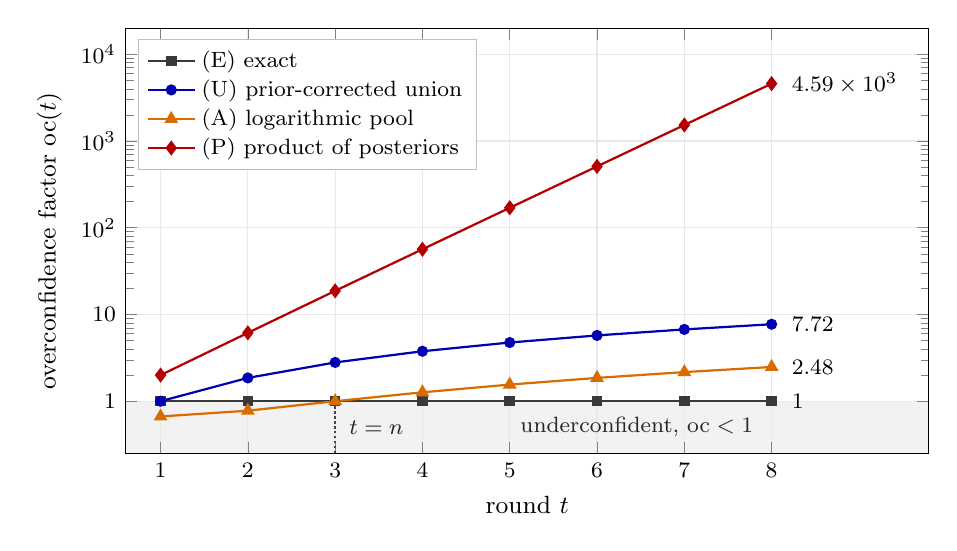
\begin{tikzpicture}
  \begin{semilogyaxis}[name=oc, scale only axis, width=10.2cm, height=5.4cm, set layers,
      xmin=0.6, xmax=9.8, ymin=0.25, ymax=2e4,
      xtick={1,...,8}, ytick={1,10,100,1000,10000}, yticklabels={$1$,$10$,$10^2$,$10^3$,$10^4$},
      xlabel={round $t$}, ylabel={overconfidence factor $\mathrm{oc}(t)$},
      grid=major, grid style={gray!18},
      legend style={font=\footnotesize, at={(0.015,0.975)}, anchor=north west, draw=gray!50, fill=white,
        cells={anchor=west}, row sep=-1pt},
      every axis label/.style={font=\small}, tick label style={font=\footnotesize}]
    \begin{pgfonlayer}{axis background}
      \fill[gray!10] (axis cs:0.6,0.25) rectangle (axis cs:9.8,1);
    \end{pgfonlayer}
    \addplot[gray!45!black, thick, mark=square*, mark size=1.5pt] coordinates {(1,1) (2,1) (3,1) (4,1) (5,1) (6,1) (7,1) (8,1)};
    \addlegendentry{(E) exact}
    \addplot[blue!70!black, thick, mark=*, mark size=1.6pt] coordinates {(1,1) (2,1.8571) (3,2.8) (4,3.7692) (5,4.75) (6,5.7368) (7,6.7273) (8,7.72)};
    \addlegendentry{(U) prior-corrected union}
    \addplot[orange!85!black, thick, mark=triangle*, mark size=2.1pt] coordinates {(1,0.66667) (2,0.77778) (3,1) (4,1.2667) (5,1.5556) (6,1.8571) (7,2.1667) (8,2.4815)};
    \addlegendentry{(A) logarithmic pool}
    \addplot[red!70!black, thick, mark=diamond*, mark size=2.1pt] coordinates {(1,2) (2,6.1429) (3,18.727) (4,56.522) (5,169.92) (6,510.12) (7,1530.7) (8,4592.5)};
    \addlegendentry{(P) product of posteriors}
    % values at t = 8
    \node[font=\footnotesize, anchor=west] at (axis cs:8.12,4592.5) {$4.59\times10^3$};
    \node[font=\footnotesize, anchor=west] at (axis cs:8.12,7.72) {$7.72$};
    \node[font=\footnotesize, anchor=west] at (axis cs:8.12,2.4815) {$2.48$};
    \node[font=\footnotesize, anchor=west] at (axis cs:8.12,1) {$1$};
    % (A) is calibrated at t = n = 3
    \draw[gray!55!black, densely dotted, thick] (axis cs:3,0.25) -- (axis cs:3,1);
    \node[font=\footnotesize, gray!30!black, anchor=west] at (axis cs:3.05,0.5) {$t=n$};
    \node[font=\footnotesize, gray!30!black, anchor=east] at (axis cs:7.9,0.5) {underconfident, $\mathrm{oc}<1$};
  \end{semilogyaxis}
\end{tikzpicture}

  \caption{\textbf{Overconfidence of a record rebuilt from its readers' posteriors.} The overconfidence factor $\mathrm{oc}(t)$ of \cref{tab:hie-records}, the mean-square error of the record's mean times its claimed precision, against the round $t$ on a logarithmic scale for the four aggregation rules of \cref{prop:hie-literal-records}, with three members of unit information and $\Lambda_\circ=1$; the shaded band is $\mathrm{oc}<1$. Exact counting (E) stays at $1$. The prior-corrected union (U) is exact after one round and then grows like $t$, to $7.72$ at $t=8$. The logarithmic pool (A) is underconfident for $t<n$, with $\mathrm{oc}=0.667$ and $0.778$, reaches $\mathrm{oc}=1$ at $t=n=3$ and then grows like $t/n$, to $2.48$. The product of posteriors (P) grows like $n^t$, to $4.59\times10^3$. Over the eight rounds every rule keeps the mean-square error between $1/4$ and $1/3$, so the growth is that of the claimed precision, which at $t=8$ is $25$, $9$ and $16401$ under (U), (A) and (P) against the exact $4$.}
  \label{fig:hie-overconfidence}
\end{figure}

In a changing world a record that is read by memoryless members as their prior and aggregated by rule (U) relative to its prediction equals the centralized Kalman filter, under the hypotheses stated there (Supplement, \cref{prop:hie-record-filter}).

Across levels, literal reading at every level of a scalar tree with unit noiseless links ($\mathsf G=1$, $\Psi=0$) counts a member's own datum once more for each level above the member, and a shortcut to the top that is fused as an independent prior counts the prior and every other datum twice (Supplement, \cref{prop:hie-depth}; see also \cref{rem:hie-literal-consensus,rem:hie-gauge} there).

\subsection{Records as top-down channels}\label{sec:hie-records}

Records that members write and read, such as archives, ledgers and shared notes, are top-down channels. Throughout this subsection a collective $C$ of $n$ members has one global record $z$, read by every member with weight $\beta$ in place of self-weight ($\upsilon=0$) and written by the members' mean with weight $\omega$, with decay $\delta$. In the continuous-time form of \cref{def:fw-record-model} with a uniform kernel on $C$, the global record of \cref{sec:sca-time}, the world-conditional errors obey
\begin{equation}\label{eq:hie-record}
\mathrm de_i=-\Bigl[(\varepsilon+\beta)e_i+\sum_ja_{ij}(e_i-e_j)-\beta z\Bigr]\mathrm dt+\sqrt{2q}\mathrm d\mathsf B_i,\qquad\mathrm dz=-\Bigl[(\omega+\delta)z-\frac\omega n\sum_{i\in C}e_i\Bigr]\mathrm dt+\sqrt{2q_z}\mathrm d\mathsf B_z,
\end{equation}
with symmetric couplings $a_{ij}=a_{ji}\ge0$. We write $L_C$ for the Laplacian of the couplings inside $C$, $\mathcal R=\beta/\omega$, and $\mathsf R=\bigl(\begin{smallmatrix}\varepsilon+\beta&-\beta\\-\omega&\omega+\delta\end{smallmatrix}\bigr)$ for the matrix of the reduced record model of \cref{prop:sca-records}, with eigenvalues $\mathsf r_-\le\mathsf r_+$; the smaller is the effective leak $\varepsilon_{\mathrm{rec}}$.

\begin{proposition}[Drift timescale separation with a global record]\label{prop:hie-record-gain}
Let the exterior of $C$ be held fixed, with uniform cut couplings absorbed into $\varepsilon$.
\begin{enumerate}
\item[(a)] The drift spectrum is $\{\mathsf r_-,\mathsf r_+\}\cup\{\varepsilon+\beta+\lambda_k(L_C):k\ge2\}$, with $\mathsf r_\pm=\frac12\bigl[\varepsilon+\beta+\omega+\delta\pm((\varepsilon+\beta-\omega-\delta)^2+4\beta\omega)^{1/2}\bigr]$; without the record it is $\{\varepsilon\}\cup\{\varepsilon+\lambda_k(L_C):k\ge2\}$.
\item[(b)] The ratio of the second-smallest to the smallest rate changes by the factor
\begin{equation}\label{eq:hie-gain}
\mathsf g_{\mathrm{sep}}=\frac{\varepsilon}{\mathsf r_-}\cdot\frac{\min\{\mathsf r_+,\varepsilon+\beta+\lambda_2(L_C)\}}{\varepsilon+\lambda_2(L_C)}.
\end{equation}
Let $\mathsf g_\times=(1+\mathcal R)(1+\beta/(\varepsilon+\lambda_2(L_C)))$, the product of the record's memory factor and the reading factor.
\item[(c)] For $\delta=0$, $\varepsilon/\mathsf r_-\in[1+\mathcal R,1+\mathcal R+\varepsilon/\omega]$, and if $\lambda_2(L_C)+\varepsilon/(1+\mathcal R)\le\omega$, then $\mathsf g_\times\le\mathsf g_{\mathrm{sep}}\le(1+\mathcal R+\varepsilon/\omega)(1+\beta/(\varepsilon+\lambda_2(L_C)))$.
\item[(d)] If $\mathsf r_+<\varepsilon+\beta+\lambda_2(L_C)$, the second-slowest mode is the exchange between the members' mean and the record, and for every $\delta\ge0$
\begin{equation}\label{eq:hie-gain-ratio}
\frac{\mathsf g_{\mathrm{sep}}}{\mathsf g_\times}=\frac{\varepsilon/\mathsf r_-}{1+\mathcal R}\cdot\frac{\mathsf r_+}{\varepsilon+\beta+\lambda_2(L_C)}<1+\frac{\varepsilon}{\omega(1+\mathcal R)};
\end{equation}
for $\delta=0$ the ratio tends to $(\beta+\omega)/(\beta+\lambda_2(L_C))$ as $\varepsilon\to0$, which is below one when $\omega<\lambda_2(L_C)$.
\item[(e)] For $\delta>0$, $\varepsilon/\mathsf r_-\ge\varepsilon(1+\mathcal R)/(\varepsilon+\mathcal R\delta)$, a bound that exceeds one if and only if $\delta<\varepsilon$.
\end{enumerate}
\end{proposition}
% src: H2-P6; HC_critic V3 (ratio bound (d) replaces the lane's "the gain is smaller")

Proof in \cref{app:hie}; checked in \cref{chk:hie-record-drift}. The record multiplies the memory of the collective mode by about $1+\mathcal R$ and adds $\beta$ to the rate of every internal disagreement, but the product of the two factors is the separation gain only when the record is written faster than the members mix; on a ring of ten members with neighbor coupling $1$, $\varepsilon=0.01$, $\beta=0.2$ and $\omega=0.1$ the gain is $2.40$ against the product $4.53$. For $\delta=0$ a weakly read record lowers the separation of the joint drift spectrum of members and record: when $\mathsf r_+<\varepsilon+\beta+\lambda_2(L_C)$ the identity $\mathsf r_+\mathsf r_-=\varepsilon\omega$ turns \eqref{eq:hie-gain} into $\mathsf g_{\mathrm{sep}}=\mathsf r_+^2/(\omega(\varepsilon+\lambda_2(L_C)))$, and since $\mathsf r_+$ increases with $\beta$, $\mathsf g_{\mathrm{sep}}<1$ exactly for $\beta<(\mathsf r_\circ-\varepsilon)(\mathsf r_\circ-\omega)/\mathsf r_\circ$ with $\mathsf r_\circ=(\omega(\varepsilon+\lambda_2(L_C)))^{1/2}$, a nonempty range exactly when $\max\{\varepsilon,\omega\}<\mathsf r_\circ$, because the second-slowest rate is then the exchange rate $\mathsf r_+$ of the members' mean and the record rather than an internal rate; on the ring of ten this range is $\beta<0.0930$, and $\mathsf g_{\mathrm{sep}}\to\omega/(\varepsilon+\lambda_2(L_C))=0.255$ as $\beta\to0$. In that limit $\mathsf r_+$ tends to the record's own rate $\omega$, here larger than $\varepsilon$, and the members' own rates tend to those without the record, so the lowered separation is a property of the joint spectrum, in which a record that is barely read contributes its own rate, and not a change in the members' dynamics. The memory factor also extends identity under turnover.

\begin{corollary}[Identity gain from a member-written record]\label{cor:hie-identity}
In the setting and under the hypotheses of \cref{prop:agy-identity}, namely turnover rate $g>0$, newcomer noise of positive finite variance and $\det\mathsf A>0$, with newcomer fidelity $\mathsf f$, put $\tilde\varepsilon=\varepsilon+g(1-\mathsf f)$, $\tilde\beta=\beta+g\mathsf f$ and $\tilde{\mathcal R}=\tilde\beta/\omega$. The identity time with the record is that of the pair $(\bar\mu,z)$ of \cref{prop:agy-identity}(a), and for $\tilde\beta>0$ it is also that of the members' mean $\bar\mu$. Divided by the identity time without the record, with newcomers copying the members' mean with the same fidelity, it lies in $[1+\tilde{\mathcal R},1+\tilde{\mathcal R}+\tilde\varepsilon/\omega]$ for $\delta=0$, and is at least $\tilde\varepsilon(1+\tilde{\mathcal R})/(\tilde\varepsilon+\tilde{\mathcal R}\delta)$ for every $\delta\ge0$. For $\tilde\beta=0$ the record is unread, the members' mean has the same identity time with and without it, and a ratio above $1$ concerns the record alone.
\end{corollary}
% src: H2-C1; identification with prop:agy-identity(a) re-derived and checked in the verification round (pvrf_hie)

Proof in \cref{app:hie}; checked in \cref{chk:hie-record-drift}. For a convention, which no member senses, the record is pure gain; for a grounded coordinate it is a top-down prior on the world, paid for in shared error. In the scalar level-0 network of \cref{def:fw-level0} with exact code models, let a collective $C$ closed under attention, with common sensing gain $k^s$, read with gain $\beta$ and read noise $\nu_z$ a record that predicts the world from the members' predicted means, $z(t+1)=F[(1-\omega)z(t)+\omega\bar m_C(t)]$, so that its error $e_z=z-\eta$ joins the members' errors in the error recursion.

\begin{lemma}[Records are blind to shared error and slow its correction]\label{lem:hie-record-blind}
\leavevmode
\begin{enumerate}
\item[(a)] Adding a common process $x(t)$ to every member's error and to the record's error leaves every social innovation $y_{ij}-m_i=e_j-e_i+\nu_{ij}$ and every top-down innovation $z+\nu_z-m_i=e_z-e_i+\nu_z$ unchanged, and shifts every sensory innovation $s_i-m_i=v_i-e_i$ by $-x(t)$: no statistic of social and top-down innovations carries information about a misconception that the members share with their record.
\item[(b)] Let $1-k^s-\beta-\sum_jk_{ij}\ge0$ and $\beta+\omega\le1$, and let $\mathsf N=\bigl(\begin{smallmatrix}1-k^s-\beta&\beta\\\omega&1-\omega\end{smallmatrix}\bigr)$. A common shift $x_0$ at round $0$ evolves, other inputs held fixed, as $x_0(\mathsf f_t\one_C,\mathsf f^z_t)$ with $(\mathsf f_t,\mathsf f^z_t)^\top=(F\mathsf N)^t(1,1)^\top$, coefficients unrelated to the newcomer fidelity $\mathsf f$ of \cref{cor:hie-identity}, and $\mathsf f_t\ge(F(1-k^s))^t$. If $\beta>0$, its asymptotic decay factor per round is $F\mathsf m_1$, with $\mathsf m_1$ the larger eigenvalue of $\mathsf N$ and $1-\mathsf m_1=\varepsilon_{\mathrm{rec}}\in[k^s/(1+\mathcal R+k^s/\omega),k^s/(1+\mathcal R)]$: the record slows the grounding-driven correction of a shared misconception from $k^s$ per round to at most $k^s/(1+\mathcal R)$.
\end{enumerate}
\end{lemma}
% src: H2-L2; extends lem:mis-social-blind

Proof in \cref{app:hie}. Part (a) extends \cref{lem:mis-social-blind} to top-down innovations: a record written by the members agrees with them about every error they share.

\begin{theorem}[The shared-error floor grows with top-down reading]\label{thm:hie-floor}
Let the world be stationary with $0<F<1$ and $Q>0$, the local noises independent of the world innovations, and $\beta,\omega>0$, in the setting of \cref{lem:hie-record-blind}(b). Every member's stationary mean-square error satisfies $\E e_i^2\ge Q\mathsf F_{\mathrm{com}}$, where $\mathsf F_{\mathrm{com}}=\sum_{s\ge0}\mathsf f_s^2$ is the variance factor of the common mode, and:
\begin{enumerate}
\item[(a)] with $\mathsf m_1>\mathsf m_2$ the eigenvalues of $\mathsf N$, $\mathsf c_1=(1-k^s-\mathsf m_2)/(\mathsf m_1-\mathsf m_2)>0$ and $\mathsf c_2=(\mathsf m_1-1+k^s)/(\mathsf m_1-\mathsf m_2)\ge0$,
\begin{equation}\label{eq:hie-floor}
\mathsf F_{\mathrm{com}}=\frac{\mathsf c_1^2}{1-F^2\mathsf m_1^2}+\frac{2\mathsf c_1\mathsf c_2}{1-F^2\mathsf m_1\mathsf m_2}+\frac{\mathsf c_2^2}{1-F^2\mathsf m_2^2};
\end{equation}
\item[(b)] $\mathsf F_{\mathrm{com}}\ge1/(1-F^2(1-k^s)^2)$, the factor of the floor of \cref{prop:mis-mse-floor} without the record, strictly when $k^s>0$;
\item[(c)] $\mathsf F_{\mathrm{com}}$ is nondecreasing in $\beta$ and nonincreasing in $\omega$;
\item[(d)] $\mathsf F_{\mathrm{com}}\ge\mathsf c_1^2/(1-F^2(1-k^s/(1+\mathcal R))^2)$, and $\mathsf c_1\to1$ as $k^s\to0$;
\item[(e)] $\mathsf F_{\mathrm{com}}<(1+\mathcal R)/(1-F^2(1-k^s)^2)$, and at fixed $\beta$ and $\omega$, if $k^s\to0$ and $F\to1$ with $(1-F)/k^s\to\mathsf y\in[0,\infty)$, then $\mathsf F_{\mathrm{com}}(1-F^2(1-k^s)^2)\to(1+\mathsf y)(1+\mathcal R)/(1+\mathsf y(1+\mathcal R))$, which is $1+\mathcal R$ at $\mathsf y=0$.
\end{enumerate}
\end{theorem}
% src: H2-T2; HC_critic V3; (e) proved in the verification round (pvrf_hie_sym, pvrf_hie), replacing the numerical support of "up to 1+R"

\begin{figure}[!t]
  \centering
  % Figure: records buy memory with shared error (prop:hie-record-gain, thm:hie-floor).
% (a) Ring of n = 10 members with neighbor coupling 1, so lambda_k(L_C) = 2 - 2cos(2 pi k/10): 0.38197, 1.38197,
%     2.61803 and 3.61803 twice each and 4 once for k >= 2; eps = 0.01, omega = 0.1, delta = 0, one global record
%     read with weight beta in place of self-weight; 51 values of beta in [0, 1].
%     Upper plot: drift spectrum of eq:hie-record by prop:hie-record-gain(a), the rates
%       r_pm = (1/2)[eps + beta + omega + delta +- ((eps + beta - omega - delta)^2 + 4 beta omega)^(1/2)]
%     of the members' mean and the record, and the internal rates eps + beta + lambda_k(L_C), k >= 2. The
%     eigenvalues of the full 11 x 11 drift agree with these to a relative deviation 8.4e-13.
%     Lower plot: the separation gain g_sep of eq:hie-gain and the product g_x = (1 + R)(1 + beta/(eps + lambda_2(L_C))),
%     R = beta/omega; g_sep from the full spectrum agrees with eq:hie-gain to 8.4e-13. Since omega < lambda_2(L_C),
%     r_+ < eps + beta + omega < eps + beta + lambda_2(L_C) for every beta, so the second-slowest mode is the exchange
%     of mean and record, and g_sep/g_x stays within 3.1 percent of its eps -> 0 limit (beta + omega)/(beta + lambda_2)
%     of prop:hie-record-gain(d), at most 0.803. At beta = 0.2: r_- = 0.003260 against eps/(1 + R) = 0.003333,
%     r_+ = 0.3067, g_sep = 2.400 against g_x = 4.531, the values of chk:hie-record-drift. g_sep -> omega/(eps +
%     lambda_2) = 0.255 as beta -> 0, g_sep = 1 at beta = 0.0930, and g_sep = 31.38 against g_x = 39.06 at beta = 1.
% (b) Common-mode factor F_com of eq:hie-floor, F_com = c_1^2/(1 - F^2 m_1^2) + 2 c_1 c_2/(1 - F^2 m_1 m_2)
%     + c_2^2/(1 - F^2 m_2^2) with m_1 > m_2 the eigenvalues of N = [[1 - k^s - beta, beta], [omega, 1 - omega]],
%     divided by its value 1/(1 - F^2 (1 - k^s)^2) without the record (thm:hie-floor(b)), against 1 + R with
%     beta = R omega; 46 points per curve, logarithmic axes. F = 0.9, 0.99, 0.999 at k^s = 0.05, omega = 0.1
%     (beta from 0 to 0.9); F = 0.9999 at k^s = 0.02, omega = 0.05 (beta from 0 to 0.45). The closed form agrees
%     with the series sum_s f_s^2 and with a Stein-equation solve to 2.2e-13. Marked: 1.113, 1.936, 2.553 for
%     F = 0.9, 0.99, 0.999 at beta = 0.2 (1 + R = 3), and 8.240 for F = 0.9999 at beta = 0.4 (1 + R = 9), where
%     F_com = 207.1 against 25.13, the values of chk:hie-record-drift. At 1 + R = 10 the ratios are 1.267, 3.620,
%     7.892 and 9.141. No curve exceeds the dashed line 1 + R. Data are embedded as computed, in double precision.
\begin{tikzpicture}
  \pgfplotsset{recframe/.style={scale only axis, width=6.1cm, grid=major, grid style={gray!18},
      every axis label/.style={font=\small}, tick label style={font=\footnotesize}},
    leftlabel/.style={every axis y label/.style={font=\small, rotate=90, at={(axis description cs:-0.165,0.5)}, anchor=south}}}
  % panel (a), upper plot: drift spectrum
  \begin{semilogyaxis}[recframe, leftlabel, name=spec, height=4.3cm, xmin=0, xmax=1, ymin=3e-4, ymax=40,
      xticklabels={}, ytick={1e-3,1e-2,1e-1,1,10}, ylabel={drift rate}]
    \addplot[gray!55, thick] coordinates {(0,0.39197) (0.02,0.41197) (0.04,0.43197) (0.06,0.45197) (0.08,0.47197) (0.1,0.49197) (0.12,0.51197) (0.14,0.53197) (0.16,0.55197) (0.18,0.57197) (0.2,0.59197) (0.22,0.61197) (0.24,0.63197) (0.26,0.65197) (0.28,0.67197) (0.3,0.69197) (0.32,0.71197) (0.34,0.73197) (0.36,0.75197) (0.38,0.77197) (0.4,0.79197) (0.42,0.81197) (0.44,0.83197) (0.46,0.85197) (0.48,0.87197) (0.5,0.89197) (0.52,0.91197) (0.54,0.93197) (0.56,0.95197) (0.58,0.97197) (0.6,0.99197) (0.62,1.012) (0.64,1.032) (0.66,1.052) (0.68,1.072) (0.7,1.092) (0.72,1.112) (0.74,1.132) (0.76,1.152) (0.78,1.172) (0.8,1.192) (0.82,1.212) (0.84,1.232) (0.86,1.252) (0.88,1.272) (0.9,1.292) (0.92,1.312) (0.94,1.332) (0.96,1.352) (0.98,1.372) (1,1.392)};
    \addplot[gray!55, thick] coordinates {(0,1.392) (0.02,1.412) (0.04,1.432) (0.06,1.452) (0.08,1.472) (0.1,1.492) (0.12,1.512) (0.14,1.532) (0.16,1.552) (0.18,1.572) (0.2,1.592) (0.22,1.612) (0.24,1.632) (0.26,1.652) (0.28,1.672) (0.3,1.692) (0.32,1.712) (0.34,1.732) (0.36,1.752) (0.38,1.772) (0.4,1.792) (0.42,1.812) (0.44,1.832) (0.46,1.852) (0.48,1.872) (0.5,1.892) (0.52,1.912) (0.54,1.932) (0.56,1.952) (0.58,1.972) (0.6,1.992) (0.62,2.012) (0.64,2.032) (0.66,2.052) (0.68,2.072) (0.7,2.092) (0.72,2.112) (0.74,2.132) (0.76,2.152) (0.78,2.172) (0.8,2.192) (0.82,2.212) (0.84,2.232) (0.86,2.252) (0.88,2.272) (0.9,2.292) (0.92,2.312) (0.94,2.332) (0.96,2.352) (0.98,2.372) (1,2.392)};
    \addplot[gray!55, thick] coordinates {(0,2.628) (0.02,2.648) (0.04,2.668) (0.06,2.688) (0.08,2.708) (0.1,2.728) (0.12,2.748) (0.14,2.768) (0.16,2.788) (0.18,2.808) (0.2,2.828) (0.22,2.848) (0.24,2.868) (0.26,2.888) (0.28,2.908) (0.3,2.928) (0.32,2.948) (0.34,2.968) (0.36,2.988) (0.38,3.008) (0.4,3.028) (0.42,3.048) (0.44,3.068) (0.46,3.088) (0.48,3.108) (0.5,3.128) (0.52,3.148) (0.54,3.168) (0.56,3.188) (0.58,3.208) (0.6,3.228) (0.62,3.248) (0.64,3.268) (0.66,3.288) (0.68,3.308) (0.7,3.328) (0.72,3.348) (0.74,3.368) (0.76,3.388) (0.78,3.408) (0.8,3.428) (0.82,3.448) (0.84,3.468) (0.86,3.488) (0.88,3.508) (0.9,3.528) (0.92,3.548) (0.94,3.568) (0.96,3.588) (0.98,3.608) (1,3.628)};
    \addplot[gray!55, thick] coordinates {(0,3.628) (0.02,3.648) (0.04,3.668) (0.06,3.688) (0.08,3.708) (0.1,3.728) (0.12,3.748) (0.14,3.768) (0.16,3.788) (0.18,3.808) (0.2,3.828) (0.22,3.848) (0.24,3.868) (0.26,3.888) (0.28,3.908) (0.3,3.928) (0.32,3.948) (0.34,3.968) (0.36,3.988) (0.38,4.008) (0.4,4.028) (0.42,4.048) (0.44,4.068) (0.46,4.088) (0.48,4.108) (0.5,4.128) (0.52,4.148) (0.54,4.168) (0.56,4.188) (0.58,4.208) (0.6,4.228) (0.62,4.248) (0.64,4.268) (0.66,4.288) (0.68,4.308) (0.7,4.328) (0.72,4.348) (0.74,4.368) (0.76,4.388) (0.78,4.408) (0.8,4.428) (0.82,4.448) (0.84,4.468) (0.86,4.488) (0.88,4.508) (0.9,4.528) (0.92,4.548) (0.94,4.568) (0.96,4.588) (0.98,4.608) (1,4.628)};
    \addplot[gray!55, thick] coordinates {(0,4.01) (0.02,4.03) (0.04,4.05) (0.06,4.07) (0.08,4.09) (0.1,4.11) (0.12,4.13) (0.14,4.15) (0.16,4.17) (0.18,4.19) (0.2,4.21) (0.22,4.23) (0.24,4.25) (0.26,4.27) (0.28,4.29) (0.3,4.31) (0.32,4.33) (0.34,4.35) (0.36,4.37) (0.38,4.39) (0.4,4.41) (0.42,4.43) (0.44,4.45) (0.46,4.47) (0.48,4.49) (0.5,4.51) (0.52,4.53) (0.54,4.55) (0.56,4.57) (0.58,4.59) (0.6,4.61) (0.62,4.63) (0.64,4.65) (0.66,4.67) (0.68,4.69) (0.7,4.71) (0.72,4.73) (0.74,4.75) (0.76,4.77) (0.78,4.79) (0.8,4.81) (0.82,4.83) (0.84,4.85) (0.86,4.87) (0.88,4.89) (0.9,4.91) (0.92,4.93) (0.94,4.95) (0.96,4.97) (0.98,4.99) (1,5.01)};
    \addplot[green!45!black, thick] coordinates {(0,0.1) (0.02,0.12179) (0.04,0.14301) (0.06,0.1639) (0.08,0.18458) (0.1,0.20512) (0.12,0.22557) (0.14,0.24593) (0.16,0.26624) (0.18,0.28651) (0.2,0.30674) (0.22,0.32694) (0.24,0.34712) (0.26,0.36728) (0.28,0.38742) (0.3,0.40755) (0.32,0.42766) (0.34,0.44777) (0.36,0.46786) (0.38,0.48795) (0.4,0.50803) (0.42,0.52811) (0.44,0.54818) (0.46,0.56824) (0.48,0.5883) (0.5,0.60836) (0.52,0.62841) (0.54,0.64846) (0.56,0.6685) (0.58,0.68855) (0.6,0.70859) (0.62,0.72863) (0.64,0.74866) (0.66,0.7687) (0.68,0.78873) (0.7,0.80876) (0.72,0.82879) (0.74,0.84882) (0.76,0.86885) (0.78,0.88887) (0.8,0.9089) (0.82,0.92892) (0.84,0.94895) (0.86,0.96897) (0.88,0.98899) (0.9,1.009) (0.92,1.029) (0.94,1.049) (0.96,1.0691) (0.98,1.0891) (1,1.1091)};
    \addplot[blue!70!black, thick] coordinates {(0,0.01) (0.02,0.0082109) (0.04,0.0069926) (0.06,0.0061013) (0.08,0.0054176) (0.1,0.0048751) (0.12,0.0044333) (0.14,0.0040661) (0.16,0.003756) (0.18,0.0034903) (0.2,0.0032601) (0.22,0.0030587) (0.24,0.0028809) (0.26,0.0027227) (0.28,0.0025812) (0.3,0.0024537) (0.32,0.0023383) (0.34,0.0022333) (0.36,0.0021374) (0.38,0.0020494) (0.4,0.0019684) (0.42,0.0018936) (0.44,0.0018242) (0.46,0.0017598) (0.48,0.0016998) (0.5,0.0016438) (0.52,0.0015913) (0.54,0.0015421) (0.56,0.0014959) (0.58,0.0014523) (0.6,0.0014113) (0.62,0.0013724) (0.64,0.0013357) (0.66,0.0013009) (0.68,0.0012679) (0.7,0.0012365) (0.72,0.0012066) (0.74,0.0011781) (0.76,0.0011509) (0.78,0.001125) (0.8,0.0011002) (0.82,0.0010765) (0.84,0.0010538) (0.86,0.001032) (0.88,0.0010111) (0.9,0.00099107) (0.92,0.00097179) (0.94,0.00095325) (0.96,0.0009354) (0.98,0.0009182) (1,0.00090163)};
    \draw[gray!60!black, densely dotted, thick] (axis cs:0,0.01) -- (axis cs:1,0.01);
    \draw[black!55, dashed] (axis cs:0.2,3e-4) -- (axis cs:0.2,40);
    \addplot[only marks, mark=*, mark size=1.6pt, blue!70!black] coordinates {(0.2,0.0032601)};
    \addplot[only marks, mark=*, mark size=1.6pt, green!45!black] coordinates {(0.2,0.30674)};
    \node[font=\footnotesize, gray!35!black, anchor=south west] at (axis cs:0.25,5.5) {$\varepsilon+\beta+\lambda_k(L_C)$, $k\ge2$};
    \node[font=\footnotesize, green!35!black, anchor=north west] at (axis cs:0.5,0.46) {$\mathsf r_+$};
    \node[font=\footnotesize, blue!60!black, anchor=north east] at (axis cs:0.75,1.0e-3) {$\mathsf r_-$};
    \node[font=\footnotesize, gray!30!black, anchor=south east] at (axis cs:0.98,0.01) {$\varepsilon$, no record};
  \end{semilogyaxis}
  \node[font=\small\bfseries, anchor=south east] at ($(spec.north west)+(-0.25cm,0.15cm)$) {(a)};
  % panel (a), lower plot: separation gain
  \begin{semilogyaxis}[recframe, leftlabel, name=gain, height=2.75cm, at={($(spec.south west)+(0,-0.25cm)$)}, anchor=north west,
      xmin=0, xmax=1, ymin=0.2, ymax=60, ytick={0.3,1,3,10,30}, log ticks with fixed point,
      xlabel={read weight $\beta$}, ylabel={gain}]
    \draw[gray!60!black, densely dotted, thick] (axis cs:0,1) -- (axis cs:1,1);
    \draw[black!55, dashed] (axis cs:0.2,0.2) -- (axis cs:0.2,60);
    \addplot[gray!55!black, thick, dashed] coordinates {(0,1) (0.02,1.2612) (0.04,1.5429) (0.06,1.8449) (0.08,2.1674) (0.1,2.5102) (0.12,2.8735) (0.14,3.2572) (0.16,3.6613) (0.18,4.0858) (0.2,4.5307) (0.22,4.9961) (0.24,5.4818) (0.26,5.988) (0.28,6.5145) (0.3,7.0615) (0.32,7.6289) (0.34,8.2167) (0.36,8.8249) (0.38,9.4535) (0.4,10.102) (0.42,10.772) (0.44,11.462) (0.46,12.172) (0.48,12.903) (0.5,13.654) (0.52,14.425) (0.54,15.217) (0.56,16.029) (0.58,16.862) (0.6,17.715) (0.62,18.589) (0.64,19.483) (0.66,20.397) (0.68,21.332) (0.7,22.287) (0.72,23.263) (0.74,24.259) (0.76,25.275) (0.78,26.312) (0.8,27.369) (0.82,28.447) (0.84,29.545) (0.86,30.663) (0.88,31.802) (0.9,32.961) (0.92,34.141) (0.94,35.341) (0.96,36.561) (0.98,37.802) (1,39.064)};
    \addplot[black, thick] coordinates {(0,0.25512) (0.02,0.37841) (0.04,0.52176) (0.06,0.68533) (0.08,0.86922) (0.1,1.0735) (0.12,1.2981) (0.14,1.5431) (0.16,1.8085) (0.18,2.0943) (0.2,2.4004) (0.22,2.727) (0.24,3.074) (0.26,3.4414) (0.28,3.8292) (0.3,4.2375) (0.32,4.6661) (0.34,5.1151) (0.36,5.5846) (0.38,6.0744) (0.4,6.5847) (0.42,7.1153) (0.44,7.6664) (0.46,8.2379) (0.48,8.8298) (0.5,9.4421) (0.52,10.075) (0.54,10.728) (0.56,11.401) (0.58,12.095) (0.6,12.81) (0.62,13.544) (0.64,14.3) (0.66,15.075) (0.68,15.871) (0.7,16.688) (0.72,17.524) (0.74,18.382) (0.76,19.259) (0.78,20.157) (0.8,21.076) (0.82,22.015) (0.84,22.974) (0.86,23.954) (0.88,24.954) (0.9,25.974) (0.92,27.015) (0.94,28.076) (0.96,29.158) (0.98,30.26) (1,31.383)};
    \addplot[only marks, mark=*, mark size=1.6pt, black] coordinates {(0.2,2.4004) (0.2,4.5307)};
    \node[font=\footnotesize, anchor=south east] at (axis cs:0.19,4.75) {$4.53$};
    \node[font=\footnotesize, anchor=west] at (axis cs:0.215,1.65) {$2.40$};
    \node[font=\footnotesize, gray!40!black, anchor=south east] at (axis cs:0.42,11.5) {$\mathsf g_\times$};
    \node[font=\footnotesize, anchor=north west] at (axis cs:0.8,18) {$\mathsf g_{\mathrm{sep}}$};
  \end{semilogyaxis}
  % panel (b): common-mode factor with the record over its value without
  \begin{loglogaxis}[recframe, name=floor, at={($(spec.north east)+(1.45cm,0)$)}, anchor=north west, height=7.3cm,
      clip=false, xmin=1, xmax=10, ymin=1, ymax=10, xtick={1,2,3,4,5,6,8,10}, ytick={1,2,3,4,5,6,8,10},
      log ticks with fixed point,
      xlabel={memory factor $1+\mathcal R$}, ylabel={$\mathsf F_{\mathrm{com}}(\beta)/\mathsf F_{\mathrm{com}}(0)$},
      legend style={font=\footnotesize, at={(0.03,0.97)}, anchor=north west, draw=gray!50, fill=white,
        cells={anchor=west, align=left}, row sep=-1pt}]
    \addplot[orange!70, thick] coordinates {(1,1) (1.2,1.014) (1.4,1.0275) (1.6,1.0403) (1.8,1.0525) (2,1.0641) (2.2,1.075) (2.4,1.0854) (2.6,1.0952) (2.8,1.1046) (3,1.1134) (3.2,1.1218) (3.4,1.1298) (3.6,1.1374) (3.8,1.1446) (4,1.1514) (4.2,1.158) (4.4,1.1642) (4.6,1.1702) (4.8,1.1759) (5,1.1813) (5.2,1.1865) (5.4,1.1915) (5.6,1.1963) (5.8,1.2009) (6,1.2053) (6.2,1.2095) (6.4,1.2135) (6.6,1.2175) (6.8,1.2212) (7,1.2249) (7.2,1.2284) (7.4,1.2317) (7.6,1.235) (7.8,1.2381) (8,1.2412) (8.2,1.2441) (8.4,1.2469) (8.6,1.2497) (8.8,1.2524) (9,1.2549) (9.2,1.2574) (9.4,1.2599) (9.6,1.2622) (9.8,1.2645) (10,1.2667)};
    \addlegendentry{$F=0.9$}
    \addplot[orange!90!black, thick] coordinates {(1,1) (1.2,1.0956) (1.4,1.1945) (1.6,1.2942) (1.8,1.3931) (2,1.4902) (2.2,1.585) (2.4,1.6772) (2.6,1.7665) (2.8,1.8528) (3,1.9362) (3.2,2.0168) (3.4,2.0944) (3.6,2.1693) (3.8,2.2416) (4,2.3113) (4.2,2.3785) (4.4,2.4433) (4.6,2.5059) (4.8,2.5664) (5,2.6247) (5.2,2.6811) (5.4,2.7356) (5.6,2.7883) (5.8,2.8393) (6,2.8887) (6.2,2.9365) (6.4,2.9828) (6.6,3.0276) (6.8,3.0711) (7,3.1133) (7.2,3.1542) (7.4,3.1939) (7.6,3.2324) (7.8,3.2699) (8,3.3063) (8.2,3.3417) (8.4,3.3761) (8.6,3.4096) (8.8,3.4421) (9,3.4739) (9.2,3.5047) (9.4,3.5348) (9.6,3.5641) (9.8,3.5927) (10,3.6205)};
    \addlegendentry{$F=0.99$}
    \addplot[red!75!black, thick] coordinates {(1,1) (1.2,1.1308) (1.4,1.2728) (1.6,1.4225) (1.8,1.5774) (2,1.7359) (2.2,1.8969) (2.4,2.0596) (2.6,2.2234) (2.8,2.3879) (3,2.5528) (3.2,2.7177) (3.4,2.8825) (3.6,3.0471) (3.8,3.2112) (4,3.3748) (4.2,3.5378) (4.4,3.7002) (4.6,3.8618) (4.8,4.0226) (5,4.1827) (5.2,4.3419) (5.4,4.5003) (5.6,4.6578) (5.8,4.8145) (6,4.9702) (6.2,5.125) (6.4,5.2789) (6.6,5.4319) (6.8,5.5839) (7,5.7351) (7.2,5.8853) (7.4,6.0345) (7.6,6.1829) (7.8,6.3303) (8,6.4768) (8.2,6.6224) (8.4,6.7671) (8.6,6.9109) (8.8,7.0537) (9,7.1957) (9.2,7.3368) (9.4,7.477) (9.6,7.6163) (9.8,7.7547) (10,7.8922)};
    \addlegendentry{$F=0.999$}
    \addplot[red!40!black, thick] coordinates {(1,1) (1.2,1.1466) (1.4,1.304) (1.6,1.4689) (1.8,1.6391) (2,1.8132) (2.2,1.9902) (2.4,2.1694) (2.6,2.3502) (2.8,2.5323) (3,2.7154) (3.2,2.8993) (3.4,3.0838) (3.6,3.2687) (3.8,3.4539) (4,3.6393) (4.2,3.8249) (4.4,4.0106) (4.6,4.1963) (4.8,4.382) (5,4.5677) (5.2,4.7532) (5.4,4.9387) (5.6,5.124) (5.8,5.3091) (6,5.4941) (6.2,5.6789) (6.4,5.8634) (6.6,6.0478) (6.8,6.2319) (7,6.4158) (7.2,6.5994) (7.4,6.7828) (7.6,6.9659) (7.8,7.1487) (8,7.3313) (8.2,7.5136) (8.4,7.6956) (8.6,7.8773) (8.8,8.0587) (9,8.2398) (9.2,8.4207) (9.4,8.6012) (9.6,8.7815) (9.8,8.9614) (10,9.1411)};
    \addlegendentry{$F=0.9999$,\\$k^s=0.02$, $\omega=0.05$}
    \draw[gray!60!black, dashed] (axis cs:1,1) -- (axis cs:10,10) node[pos=0.8, sloped, above, font=\footnotesize] {$1+\mathcal R$};
    \addplot[only marks, mark=*, mark size=1.6pt, black] coordinates {(3,1.1134) (3,1.9362) (3,2.5528) (9,8.2398)};
    \node[font=\footnotesize, inner sep=1pt, anchor=west] at (axis cs:2.316,1.2285) {$1.113$};
    \node[font=\footnotesize, inner sep=1pt, anchor=west] at (axis cs:2.9271,1.757) {$1.936$};
    \node[font=\footnotesize, inner sep=1pt, anchor=west] at (axis cs:3.4300,2.6950) {$2.553$};
    \draw[gray!60!black] (axis cs:9.15,8.2398) -- (axis cs:10,8.2398) node[font=\footnotesize, text=black, inner sep=1pt, anchor=west, xshift=2pt] {$8.24$};
  \end{loglogaxis}
  \node[font=\small\bfseries, anchor=south east] at ($(floor.north west)+(-0.25cm,0.15cm)$) {(b)};
\end{tikzpicture}

  \caption{\textbf{Records buy memory with shared error.} (a) A ring of ten members with neighbor coupling $1$, $\varepsilon=0.01$, $\omega=0.1$ and $\delta=0$, and a global record read with weight $\beta$ in place of self-weight. Upper plot: the drift spectrum of \cref{prop:hie-record-gain}(a), the rates $\mathsf r_-$ of the slow collective mode and $\mathsf r_+$ of the exchange between the members' mean and the record, and the internal rates $\varepsilon+\beta+\lambda_k(L_C)$, $k\ge2$; without the record the slowest rate is $\varepsilon$ (dotted). Lower plot: the separation gain $\mathsf g_{\mathrm{sep}}$ of \eqref{eq:hie-gain} and the product $\mathsf g_\times$ of the memory factor and the reading factor (dashed). Here $\omega<\lambda_2(L_C)=0.382$: the record is written more slowly than the members mix, $\mathsf r_+$ is the second-slowest rate at every $\beta$, and the gain stays below the product, with a ratio within $3.1$ percent of its limit $(\beta+\omega)/(\beta+\lambda_2(L_C))$ as $\varepsilon\to0$ in \cref{prop:hie-record-gain}(d). For $\beta<0.093$ the gain is below one, because the second-slowest rate of the joint spectrum of members and record falls from $\varepsilon+\lambda_2(L_C)$ to $\mathsf r_+=\varepsilon+\beta+\omega-\mathsf r_-$, which tends to the record's own rate $\omega$ as $\beta\to0$, by a larger factor than the slowest rate falls from $\varepsilon$ to $\mathsf r_-$. At $\beta=0.2$ (vertical dashed line), $\mathsf r_-=0.003260$ against $\varepsilon/(1+\mathcal R)=0.003333$ and $\mathsf r_+=0.3067$, and the gain is $2.40$ against the product $4.53$. (b) The common-mode factor $\mathsf F_{\mathrm{com}}(\beta)$ of \eqref{eq:hie-floor} divided by its value $\mathsf F_{\mathrm{com}}(0)=1/(1-F^2(1-k^s)^2)$ without the record, against the memory factor $1+\mathcal R$ on logarithmic axes, for $F=0.9$, $0.99$ and $0.999$ with $k^s=0.05$ and $\omega=0.1$, and for $F=0.9999$ with $k^s=0.02$ and $\omega=0.05$. The marked values are $1.113$, $1.936$ and $2.553$ at $\beta=0.2$, where $1+\mathcal R=3$, and $8.24$ at $\beta=0.4$, where $1+\mathcal R=9$ and $\mathsf F_{\mathrm{com}}$ is $207.1$ against $25.13$. By \cref{thm:hie-floor}(e) the ratio stays below $1+\mathcal R$ (dashed) and approaches it in a persistent world with weak grounding, $k^s\to0$ with $1-F\ll k^s/(1+\mathcal R)$: the memory that the record buys in (a) is paid for in shared error.}
  \label{fig:hie-records}
\end{figure}

Proof in \cref{app:hie}; checked in \cref{chk:hie-record-drift}. By (b) and (e) the record multiplies the shared-error floor by a factor between $1$ and $1+\mathcal R$, the factor by which it lengthens memory and identity, and by (e) the factor approaches $1+\mathcal R$ in a persistent world with weak grounding, $k^s\to0$ with $1-F\ll k^s/(1+\mathcal R)$; at $F=0.9999$, $k^s=0.02$, $\beta=0.4$ and $\omega=0.05$, where $1+\mathcal R=9$, the floor grows by $8.24$. \Cref{fig:hie-records} shows both sides of the exchange: the drift spectrum and separation gain of the ring of ten under a global record, and the shared-error floor rising toward $1+\mathcal R$ as the world becomes persistent. This is the grounding tension of \cref{thm:coh-grounding-tension} across levels, and by \cref{lem:hie-record-blind} the members cannot see its price in their innovations. Records can also read records.

For a chain of nested records with read-to-write ratios $\mathcal R_k$ and leaks only at the agents, $\varepsilon_{\mathrm{rec}}\le\varepsilon/(1+\mathcal R_1+\mathcal R_1\mathcal R_2+\cdots)$, a case of a bound for records arranged on a tree (Supplement, \cref{prop:hie-nested-records}).

Drift is not precision. At the reversible record noise the precision of the population with the record as a node is diffusive, and for $\delta=0$, under the condition on $\beta$ stated there, the contrast of the collective with its record exceeds that of the collective alone by a factor that does not depend on $\omega$, so the memory factor $1+\mathcal R$ is absent from contrast (Supplement, \cref{prop:hie-record-contrast,rem:hie-memory-absent}).

Away from the reversible noise the precision with the record node can leave the diffusive class (Supplement, \cref{ex:hie-noiseless-record}, and the numerical observation \cref{obs:hie-record-window}); at that noise, for a closed population with $\delta=0$, a global record adds to the members' covariance a component common to all pairs (\cref{prop:hie-global-record}).

The weight that a top-down prior deserves is treated in the Supplement (\cref{sec:hie-balance}): under the cavity condition, weight above the Kalman value trades disagreement for shared error (\cref{prop:hie-echo-tradeoff}), and positive precision on a member-written record of a grounded coordinate strictly raises the common-mode part of every member's stationary error under the hypotheses stated there (\cref{conj:hie-top-down}), while the total error was computed only in instances (\cref{obs:hie-top-down}, a numerical observation).

\subsection{Conformity to a self-constituted prior}\label{sec:hie-conformity}

A collective prior can also act on conventions, which no member senses, and conformity is then a candidate mechanism of formation that does not rest on misreading evidence. Let agents hold conventions $\mathsf x_i\in\R$ and expected free energies
\begin{equation}\label{eq:hie-conformity}
G_i(\mathsf x)=\sum_jJ_{ij}(\mathsf x-\mathsf x_j)^2+\mathsf a_{\mathrm p}(\mathsf x-\mathsf x^0_i)^2+\beta_{\mathrm r}(\mathsf x-\bar z_{\alpha,-i})^2,
\end{equation}
up to terms free of $\mathsf x$, with exogenous symmetric attended couplings $J_{ij}=J_{ji}\ge0$, a pragmatic preference for matching attended partners; a pull $\mathsf a_{\mathrm p}>0$ toward a native convention $\mathsf x^0_i$; readership groups $\mathcal K_1,\dots,\mathcal K_{n_{\mathrm g}}$ of sizes $n_\alpha\ge2$ partitioning the agents; and the cavity reading $\bar z_{\alpha,-i}$ of the record of $i$'s group $\mathcal K_\alpha$, the mean of the other members' conventions. Write $L_J$ for the Laplacian of $J$ and $L^{\mathrm{cpl}}_\alpha$ for that of the complete graph with unit weights on $\mathcal K_\alpha$.

\begin{proposition}[Linear conformity cannot form collectives]\label{prop:hie-conformity}
\begin{enumerate}
\item[(a)] $\mathcal V(\mathsf x)=\sum_{i<j}J_{ij}(\mathsf x_i-\mathsf x_j)^2+\mathsf a_{\mathrm p}\sum_i(\mathsf x_i-\mathsf x^0_i)^2+\sum_\alpha\frac{\beta_{\mathrm r}}{n_\alpha-1}\sum_{i<j\in\mathcal K_\alpha}(\mathsf x_i-\mathsf x_j)^2$ is an exact potential. A literal reading in which the record's mean includes the agent's own convention also gives a potential game, with group coupling $\beta_{\mathrm r}(n_\alpha-1)/n_\alpha^2$ in place of $\beta_{\mathrm r}/(n_\alpha-1)$.
\item[(b)] Asynchronous revision at policy precision $\gamma$, in which a uniformly chosen agent samples $\mathsf x_i$ from $q_i\propto e^{-\gamma G_i}$, is the random-scan Gibbs sampler of $e^{-\gamma\mathcal V}$, and its unique stationary law is Gaussian with precision $\Pi=2\gamma(L_J+\mathsf a_{\mathrm p}I+\sum_\alpha\frac{\beta_{\mathrm r}}{n_\alpha-1}L^{\mathrm{cpl}}_\alpha)$, diffusive with leaks $2\gamma\mathsf a_{\mathrm p}$. There is no world to condition on, and contrast is computed from this Gibbs precision.
\item[(c)] A readership group has contrast $r(\mathcal K_\alpha)=(\mathsf a_{\mathrm p}+\lambda_2(L_{J,\alpha})+\beta_{\mathrm r}n_\alpha/(n_\alpha-1))/(\mathsf a_{\mathrm p}+\cut_J(\mathcal K_\alpha)/n_\alpha)$, with $L_{J,\alpha}$ the Laplacian of $J$ inside $\mathcal K_\alpha$: the record adds $\beta_{\mathrm r}n_\alpha/(n_\alpha-1)$ to the internal rate.
\item[(d)] The stationary law, and with it the contrast of every region, is a fixed function of $J$, $\mathsf a_{\mathrm p}$, $\beta_{\mathrm r}$ and the readership groups that does not depend on the initial state, so linear conformity selects no partition that these do not already contain. Which regions are collectives depends on the declared geometry of \cref{def:col-baseline}: no region exceeds the baseline when the comparison medium is the population itself, as under the graph clause when $\Pi$ has equal couplings on the declared edges and uniform leak; the whole population is never a collective when a group of permutations preserving the declared geometry acts transitively on the agents and on each set of pairs that the comparison medium averages (\cref{prop:col-whole-population}); and with no declared geometry only regions denser than the population average can qualify (\cref{prop:ren-exchangeable}), such as each of two disjoint cliques (\cref{rem:col-declared-geometry}).
\item[(e)] Under the deletion nulls, $J=0$ and records unread, $\Pi=2\gamma\mathsf a_{\mathrm p}I$ and no region has contrast above one. If partners and readership are redrawn independently every round, exchangeably in law and independently of the conventions, and native conventions are equal, the stationary law exists, is unique, is invariant under relabeling of the agents and singles out no partition. The exact-fusion null keeps preferences (\cref{def:agy-nulls}) and, with exogenous attention, leaves the law unchanged, so a selected structure survives it and agrees with the explanation null that predicts structure from the declared attention and readership.
\end{enumerate}
\end{proposition}
% src: H2-P10 (a), (b), (c), (e); (d) restated as H6-P10 per decision 22 (HC_critic V13); (e) restricted here to redraws renewed every round with equal native conventions

Proof in \cref{app:hie}; checked in \cref{chk:hie-conformity}. Two disjoint cliques of four with $J=1$ and $\mathsf a_{\mathrm p}=0.1$ have contrast $41.0$; each is a collective against the exchangeable baseline $35.29$, and none is when the cliques are the declared interaction graph. Conformity amplifies a partition that attention and readership already declare, and records make conventions bistable sooner.

In the code game with affine values of slope $J$ per matched attended partner, $\mathsf d$ partners and a cavity-read record of slope $\beta_{\mathrm r}$, the adoption map is bistable if and only if $\gamma(J\mathsf d+\beta_{\mathrm r})>2$, in the mean field with $h_i=0$ stated there (Supplement, \cref{prop:hie-record-bistability}). In the two-group model, under the conditions stated there, a pragmatic preference for coordinated exchange keeps the split under the translation-aware null, which is not formation (\cref{rem:hie-pragmatic}), and the strength that this needs was computed for one exact receiver at the base point (\cref{obs:hie-exact-receiver}, a numerical observation).

With attention cut at the walls between code domains on a declared ring, a domain is a collective at some admissible level under an explicit condition (Supplement, \cref{ex:hie-code-domains}); that the conformity loop forms such domains from disordered starts is conjectured (\cref{conj:hie-conformity-formation}).

\subsection{Three levels}\label{sec:hie-three}

Let $N_{\mathrm g}$ groups of $n$ members each have the internal Laplacian $L$; members leak at $\varepsilon$ and read their group record with weight $\beta_1$; group records are written by their group's mean ($\omega_1$), decay at $\delta_1$ and read the society record with weight $\beta_2$; the society record is written by the mean of the group records ($\omega_2$) and decays at $\delta_2$. Let $M$ be the continuous-time drift and $\mathcal R_l=\beta_l/\omega_l$.

\begin{theorem}[Members, groups and society]\label{thm:hie-three-levels}
\begin{enumerate}
\item[(a)] The spectrum of $M$ is the union of the member-deviation family $\{\varepsilon+\beta_1+\lambda_k(L):k\ge2\}$, each with multiplicity $N_{\mathrm g}$, the group-level family $\mathrm{spec}(\mathsf R_{\mathrm{grp}})$ with multiplicity $N_{\mathrm g}-1$, and the society family $\mathrm{spec}(\mathsf R_{\mathrm{soc}})$, where
\begin{equation}\label{eq:hie-three}
\mathsf R_{\mathrm{grp}}=\begin{pmatrix}\varepsilon+\beta_1&-\beta_1\\-\omega_1&\omega_1+\delta_1+\beta_2\end{pmatrix},\qquad\mathsf R_{\mathrm{soc}}=\begin{pmatrix}\varepsilon+\beta_1&-\beta_1&0\\-\omega_1&\omega_1+\delta_1+\beta_2&-\beta_2\\0&-\omega_2&\omega_2+\delta_2\end{pmatrix}.
\end{equation}
\item[(b)] If the read weights $\beta_1,\beta_2$ and the write weights $\omega_1,\omega_2$ are positive and the decays $\delta_1,\delta_2$ are nonnegative, all eigenvalues are real, and positive when $\varepsilon>0$.
\item[(c)] Under the hypotheses of (b), the slowest society rate is at most $(\varepsilon+\mathcal R_1\delta_1+\mathcal R_1\mathcal R_2\delta_2)/(1+\mathcal R_1+\mathcal R_1\mathcal R_2)$, and equals $\varepsilon/(1+\mathcal R_1+\mathcal R_1\mathcal R_2)+O(\varepsilon^2)$ when $\delta_1=\delta_2=0$. The slower group-level rate lies between $\det\mathsf R_{\mathrm{grp}}/\tr\mathsf R_{\mathrm{grp}}$ and twice this value, with $\det\mathsf R_{\mathrm{grp}}=\varepsilon(\omega_1+\delta_1+\beta_2)+\beta_1(\delta_1+\beta_2)$, which stays positive as $\varepsilon\to0$. The society, the differences between groups and the deviations of members therefore relax on ordered timescales whenever
\[
\frac{\varepsilon+\mathcal R_1\delta_1+\mathcal R_1\mathcal R_2\delta_2}{1+\mathcal R_1+\mathcal R_1\mathcal R_2}\ll\frac{\det\mathsf R_{\mathrm{grp}}}{\tr\mathsf R_{\mathrm{grp}}}\ll\varepsilon+\beta_1+\lambda_2(L).
\]
\end{enumerate}
\end{theorem}
% src: H2-T3, with H2-P13 for (c); positivity hypotheses of (b) stated explicitly in the verification round; ordering clause stated with the full society bound, since with delta_1 > 0 the delta = 0 value eps/(1+R1+R1R2) can be small while society and group rates coincide (proof check, chk:hie-three)

Proof in \cref{app:hie}; checked in \cref{chk:hie-three}, where five groups of ten have society rate $3.77\times10^{-4}$ against $\varepsilon=0.01$ without records and timescale separations $201$ and $135$. \Citet{kiebel2008hierarchy} impose such a separation between the levels of their model; here it follows from read and write weights.

When lower-level states have dynamics of their own, exact filtering needs a joint filter of all levels or provenance on every channel (Supplement, \cref{rem:hie-dynamic}).

\Cref{thm:hie-three-levels} is an exact block decomposition of one population, not a coarse-graining. Whether its groups are collectives of level one, and so candidate meta-agents of that level, is decided by their coarse contrast $r^{(1)}$ in the level-one coarse medium of \cref{def:col-coarse-medium} against that medium's own comparison medium, as \cref{def:col-hierarchy} requires; whether they are meta-agents depends in addition on the closure, null and agency clauses of \cref{def:agy-meta-agent}. A declared geometry for populations with record nodes is still missing (\cref{open:hie-record-contrast}). The multiplication of memory by nested records and the linear growth of literal overcounting with depth (\cref{prop:hie-nested-records,prop:hie-depth}) are what \cref{sec:ren} carries through coarse-graining.

The open problems of this section, on the two-group split under full exact fusion, contrast with record nodes, non-reversible drift and provenance in dynamic hierarchies, are stated in the Supplement (\cref{sec:hie-open}).
